\section{5 Sep 23 - Activity: Calculus of Variations and Lagrangian
Dynamics}\label{sep-23---activity-calculus-of-variations-and-lagrangian-dynamics}

In this activity, you will work through an example Lagrangian dynamics
problem. This problem is a standard one which sets up both our
understanding of the Lagrangian and the Lagrangian equations of motion,
but also coupled oscillators. The latter is a very important concept in
physics, and we will see it again in the context of waves. In addition,
we will change coordinate systems from Cartesian to polar coordinates on
our way to generalized coordinates.

We should be considering all the conceptual questions asked because
signs and distances matter in most Lagrangian problems. Setting up the
problem incorrectly is the most common mistake (we've all made it many
times) because the mathematical process is the same for every problem.

\subsection{Group Activity}\label{group-activity}

\subsubsection{Simple Harmonic Oscillator
(SHO)}\label{simple-harmonic-oscillator-sho}

\emph{Note (for this and future problems): the form of the EOM might not
look the same as the Newtonian approach, but with some algebra we can
often see that they are equivalent.}

\textbf{✅ Do this}

\begin{enumerate}
\def\labelenumi{\arabic{enumi}.}
\tightlist
\item
  Starting with the 1d energy equations (\(T\) and \(V\)) for a SHO;
  derive the equations of motion (\(m\ddot{x}=-kx\)). Use the Lagrangian
  approach. Did you get the sign right?
\end{enumerate}

\subsubsection{Canonical Coupled
Oscillators}\label{canonical-coupled-oscillators}

Let's assume you have a chain of two mass connected by springs (all with
the same \(k\)) as below.

\textbf{✅ Do this}

\begin{enumerate}
\def\labelenumi{\arabic{enumi}.}
\tightlist
\item
  Write down the energy equations for this system (using \(x_1\) and
  \(x_2\) for coordinates)
\item
  Write the Lagrangian for this system.
\item
  Derive the two equations of motion. Why should there be two equations
  of motion?
\item
  Do all the signs makes sense to you? Why?
\item
  Could you have arrived at these equations in the Newtonian framework?
  No need to do so, just sketch out how you would have done it.
\end{enumerate}

\subsubsection{Orbital Problem}\label{orbital-problem}

Consider the 2 body orbital problem of a star and an planet under the
force of gravity. Assume the star is stationary.

\textbf{✅ Do this}

\begin{enumerate}
\def\labelenumi{\arabic{enumi}.}
\tightlist
\item
  Write down the energy equations for this system using polar
  coordinates. \emph{Note: \(v^2 = \dot{r}^2 + r^2\dot{\phi}^2\)}
\item
  Write the Lagrangian.
\item
  Derive the \(r\) equation of motion. What do you notice about it's
  terms? Can you rewrite it in a Netwonian form?
\item
  Derive the \(\phi\) equation of motion. What do you notice about it's
  time derivative? Does that tell you something about a quantity of the
  motion (i.e.~a conserved quantity)? If so, what is it?
\end{enumerate}

\subsection{Additonal Examples}\label{additonal-examples}

We will discuss constrained motion together in class. The code below is
just to show you the shape of the constraints.

\subsubsection{Constrained Motion}\label{constrained-motion}

The Lagrangian framework also excels at dealing with constrained motion,
where it is usually not obvious what the constraint forces are. This is
because you can write your generalized coordinates for your system in
such a way that it contains the information

Consider a particle of mass \(m\) constrained to move on the surface of
a paraboloid \(z =  c\rho^2\) subject to a gravitational force downward,
so that the paraboloid and gravity are aligned.

\textbf{✅ Try this}

\begin{enumerate}
\def\labelenumi{\arabic{enumi}.}
\tightlist
\item
  Using cylindrical coordinates (why?), write down the equation of
  constraint. Think about where the mass must be if it's stuck on a
  paraboloid.
\item
  Write the energy contributions in cylindrical coordinates. (This is
  where you put in the constraint!)
\item
  Form the Lagrangian and find the equations of motion (there are two!)
\end{enumerate}

\begin{Shaded}
\begin{Highlighting}[]
\ImportTok{import}\NormalTok{ numpy }\ImportTok{as}\NormalTok{ np}
\ImportTok{import}\NormalTok{ matplotlib.pyplot }\ImportTok{as}\NormalTok{ plt}

\KeywordTok{def}\NormalTok{ parabaloid(x,y,alpha):}
    \CommentTok{\# function of a paraboloid in Cartesian coordinates}
    \ControlFlowTok{return}\NormalTok{ alpha }\OperatorTok{*}\NormalTok{ (x}\OperatorTok{**}\DecValTok{2} \OperatorTok{+}\NormalTok{ y}\OperatorTok{**}\DecValTok{2}\NormalTok{)}

\CommentTok{\# points of the surface to plot}
\NormalTok{x }\OperatorTok{=}\NormalTok{ np.linspace(}\OperatorTok{{-}}\FloatTok{2.8}\NormalTok{, }\FloatTok{2.8}\NormalTok{, }\DecValTok{50}\NormalTok{)}
\NormalTok{y }\OperatorTok{=}\NormalTok{ np.linspace(}\OperatorTok{{-}}\FloatTok{2.8}\NormalTok{, }\FloatTok{2.8}\NormalTok{, }\DecValTok{50}\NormalTok{)}
\NormalTok{alpha }\OperatorTok{=} \DecValTok{1}
\CommentTok{\# construct meshgrid for plotting}
\NormalTok{X, Y }\OperatorTok{=}\NormalTok{ np.meshgrid(x, y)}
\NormalTok{Z }\OperatorTok{=}\NormalTok{ parabaloid(X, Y,alpha)}

\CommentTok{\# do plotting}
\NormalTok{fig }\OperatorTok{=}\NormalTok{ plt.figure(figsize }\OperatorTok{=}\NormalTok{ (}\DecValTok{10}\NormalTok{,}\DecValTok{10}\NormalTok{))}
\NormalTok{ax }\OperatorTok{=}\NormalTok{ plt.axes(projection}\OperatorTok{=}\StringTok{\textquotesingle{}3d\textquotesingle{}}\NormalTok{)}
\NormalTok{plt.title(}\VerbatimStringTok{r"Paraboloid }\KeywordTok{(}\DecValTok{$}\CharTok{\textbackslash{}a}\VerbatimStringTok{lpha = }\DecValTok{$}\VerbatimStringTok{"} \OperatorTok{+} \BuiltInTok{str}\NormalTok{(alpha)}\OperatorTok{+} \StringTok{")"}\NormalTok{)}
\NormalTok{ax }\OperatorTok{=}\NormalTok{ plt.axes(projection}\OperatorTok{=}\StringTok{\textquotesingle{}3d\textquotesingle{}}\NormalTok{)}
\NormalTok{ax.plot\_surface(X, Y, Z, cmap}\OperatorTok{=}\StringTok{\textquotesingle{}binary\textquotesingle{}}\NormalTok{, alpha}\OperatorTok{=}\FloatTok{0.8}\NormalTok{) }
\NormalTok{ax.set\_xlim(}\OperatorTok{{-}}\DecValTok{3}\NormalTok{, }\DecValTok{3}\NormalTok{)}\OperatorTok{;}\NormalTok{ ax.set\_ylim(}\OperatorTok{{-}}\DecValTok{3}\NormalTok{, }\DecValTok{3}\NormalTok{)}\OperatorTok{;}\NormalTok{ ax.set\_zlim(}\OperatorTok{{-}}\DecValTok{1}\NormalTok{ ,}\DecValTok{15}\NormalTok{)}
\NormalTok{ax.set\_xlabel(}\StringTok{\textquotesingle{}x\textquotesingle{}}\NormalTok{)}
\NormalTok{ax.set\_ylabel(}\StringTok{\textquotesingle{}y\textquotesingle{}}\NormalTok{)}
\NormalTok{ax.set\_zlabel(}\StringTok{\textquotesingle{}z\textquotesingle{}}\NormalTok{)}
\NormalTok{plt.show()}
\end{Highlighting}
\end{Shaded}

\begin{figure}
\centering
\pandocbounded{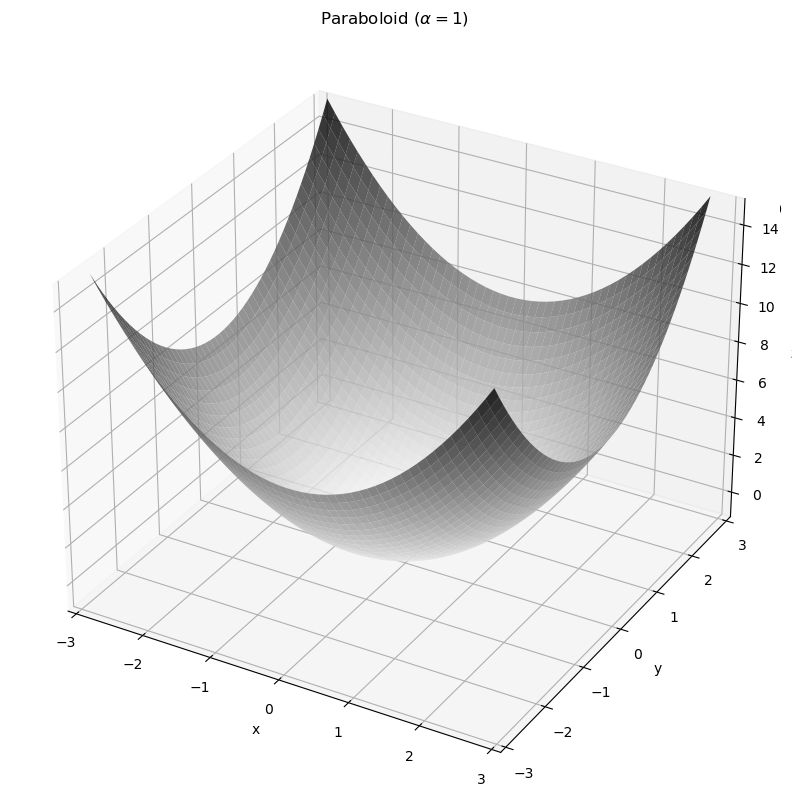
\includegraphics[keepaspectratio,alt={png}]{../images/activity-lagrange_1_activity-lagrange_1_tmp_5_0.png}}
\caption{png}
\end{figure}

\subsubsection{Roller Coaster on a Holonomic
Track}\label{roller-coaster-on-a-holonomic-track}

Consider 3 roller coaster cars of equal mass \(m\) and positions
\(x_1,x_2,x_3\), constrained to move on a one dimensional ``track''
defined by \(f(x) = x^4 -2x^2 + 1\). These cars are also constrained to
stay a distance \(d\) apart, since they are linked. We'll only worry
about that distance \(d\) in the direction for now (though a fun problem
would be to try this problem with a true fixed distance!)

\begin{Shaded}
\begin{Highlighting}[]
\NormalTok{x }\OperatorTok{=}\NormalTok{ np.arange(}\OperatorTok{{-}}\FloatTok{1.8}\NormalTok{,}\FloatTok{1.8}\NormalTok{,}\FloatTok{0.01}\NormalTok{)}
\NormalTok{track }\OperatorTok{=} \KeywordTok{lambda}\NormalTok{ x : x}\OperatorTok{**}\DecValTok{4} \OperatorTok{{-}} \DecValTok{2}\OperatorTok{*}\NormalTok{x}\OperatorTok{**}\DecValTok{2} \OperatorTok{+} \DecValTok{1}
\NormalTok{y }\OperatorTok{=}\NormalTok{ track(x)}
\NormalTok{d }\OperatorTok{=} \FloatTok{0.1}
\NormalTok{x1\_0 }\OperatorTok{=} \OperatorTok{{-}}\FloatTok{1.5}
\NormalTok{x2\_0 }\OperatorTok{=}\NormalTok{ x1\_0 }\OperatorTok{{-}}\NormalTok{ d}
\NormalTok{x3\_0 }\OperatorTok{=}\NormalTok{ x1\_0 }\OperatorTok{{-}} \DecValTok{2}\OperatorTok{*}\NormalTok{d}
\NormalTok{plt.plot(x,y, label }\OperatorTok{=} \StringTok{"track"}\NormalTok{)}
\NormalTok{plt.scatter(x1\_0,track(x1\_0),zorder }\OperatorTok{=} \DecValTok{2}\NormalTok{,label }\OperatorTok{=} \VerbatimStringTok{r"}\DecValTok{$}\VerbatimStringTok{x\_1}\DecValTok{$}\VerbatimStringTok{"}\NormalTok{)}
\NormalTok{plt.scatter(x2\_0,track(x2\_0),zorder }\OperatorTok{=} \DecValTok{2}\NormalTok{,label }\OperatorTok{=} \VerbatimStringTok{r"}\DecValTok{$}\VerbatimStringTok{x\_2}\DecValTok{$}\VerbatimStringTok{"}\NormalTok{)}
\NormalTok{plt.scatter(x3\_0,track(x3\_0),zorder }\OperatorTok{=} \DecValTok{2}\NormalTok{,label }\OperatorTok{=} \VerbatimStringTok{r"}\DecValTok{$}\VerbatimStringTok{x\_3}\DecValTok{$}\VerbatimStringTok{"}\NormalTok{)}
\NormalTok{plt.legend()}
\NormalTok{plt.grid()}
\NormalTok{plt.show()}
\end{Highlighting}
\end{Shaded}

\begin{figure}
\centering
\pandocbounded{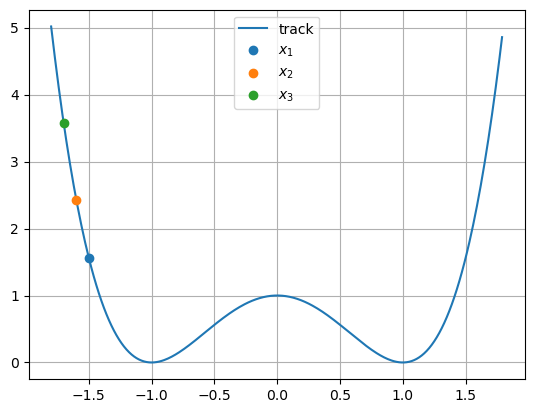
\includegraphics[keepaspectratio,alt={png}]{../images/activity-lagrange_1_activity-lagrange_1_tmp_7_0.png}}
\caption{png}
\end{figure}

\textbf{✅ Do this}

\begin{enumerate}
\def\labelenumi{\arabic{enumi}.}
\tightlist
\item
  Write down the equation(s) of constraint. How many coordinates do you
  actually need?
\item
  Write the energies of the system using your generalized coordinates.
\item
  Form the Lagrangian and find the equation(s?) of motion (how many are
  there?)
\item
  Are the dynamics of this system different that the dynamics of a
  system of just one roller coaster car?
\end{enumerate}
